\documentclass[]{ufsc-thesis-rn46-2019}

\usepackage[utf8]{inputenc} % UTF-8
\usepackage{lipsum} % Gerador de texto
\usepackage{pdfpages} % Inclui PDF externo (ficha catalográfica)

% Usado para mostrar código
\usepackage{minted}
\newmintinline[mt]{latex}{fontsize=\normalsize}
\setminted{fontsize=\tiny,linenos,xleftmargin=2em}
\setmintedinline{breaklines,breakbytokenanywhere}

%%%%%%%%%%%%%%%%%%%%%%%%%%%%%%%%%%%%%%%%%%%%%%%%%%%%%%%%%%%%%%%%%%%%
%%% Configurações da classe (dados do trabalho)                  %%%
%%%%%%%%%%%%%%%%%%%%%%%%%%%%%%%%%%%%%%%%%%%%%%%%%%%%%%%%%%%%%%%%%%%%

% Preâmbulo
\titulo{Template \LaTeX~ seguindo a RN 46/2019/CPG da UFSC}
\autor{Fulano da Silva}
% Importante! Para documentos em inglês, não use today, digite a data em
% pt_BR, como deve aparecer na folha de certificação.
\data{1 de Agosto de 2019}
\instituicao{Universidade Federal de Santa Catarina}
\programa{Programa de Pós-Graduação em Ciências da Computação}
\tese % ou \dissertacao
\local{Florianópolis} % Apenas cidade! Sem estado
\titulode{Doutor em Ciência da Computação}
\orientador{Prof. Dr. Ben Trovato}
\coorientador{Prof. Dr. Lars Thørväld}
\centro{Centro Tecnológico -- CTC}

% Membros da banca e coordenador
% As regras da BU agora exigem que Dr. apareça depois do nome
\membrobanca{Prof. Valerie Béranger, Dr.}{Universidade Federal de Santa Catarina}
\membrobanca{Prof. Aparna Patel, Dr.}{Universidade Federal de Santa Catarina}
\membrobanca{Prof. Huifen Chan, Dr.}{Universidade Federal de Santa Catarina}
% Atenção! o template da BU e o documento que apresenta as regras continua 
% usando Dr antes do nome para Orientador e Coordenador!
\coordenador{Prof. Dr. Charles Palmer, Dr.}


\begin{document}

%%%%%%%%%%%%%%%%%%%%%%%%%%%%%%%%%%%%%%%%%%%%%%%%%%%%%%%%%%%%%%%%%%%%
%%% Principais elementos pré-textuais                            %%%
%%%%%%%%%%%%%%%%%%%%%%%%%%%%%%%%%%%%%%%%%%%%%%%%%%%%%%%%%%%%%%%%%%%%

% Inicia parte pré-textual do documento capa, folha de rosto, folha de
% aprovação, aprovação, resumo, lista de tabelas, lista de figuras, etc.
\pretextual%
\imprimircapa%
\imprimirfolhaderosto*
\clearpage % força troca de página. Importante fazer isso antes do includepdf
% Ficha catalográfica deve ser gerado no site http://ficha.bu.ufsc.br/
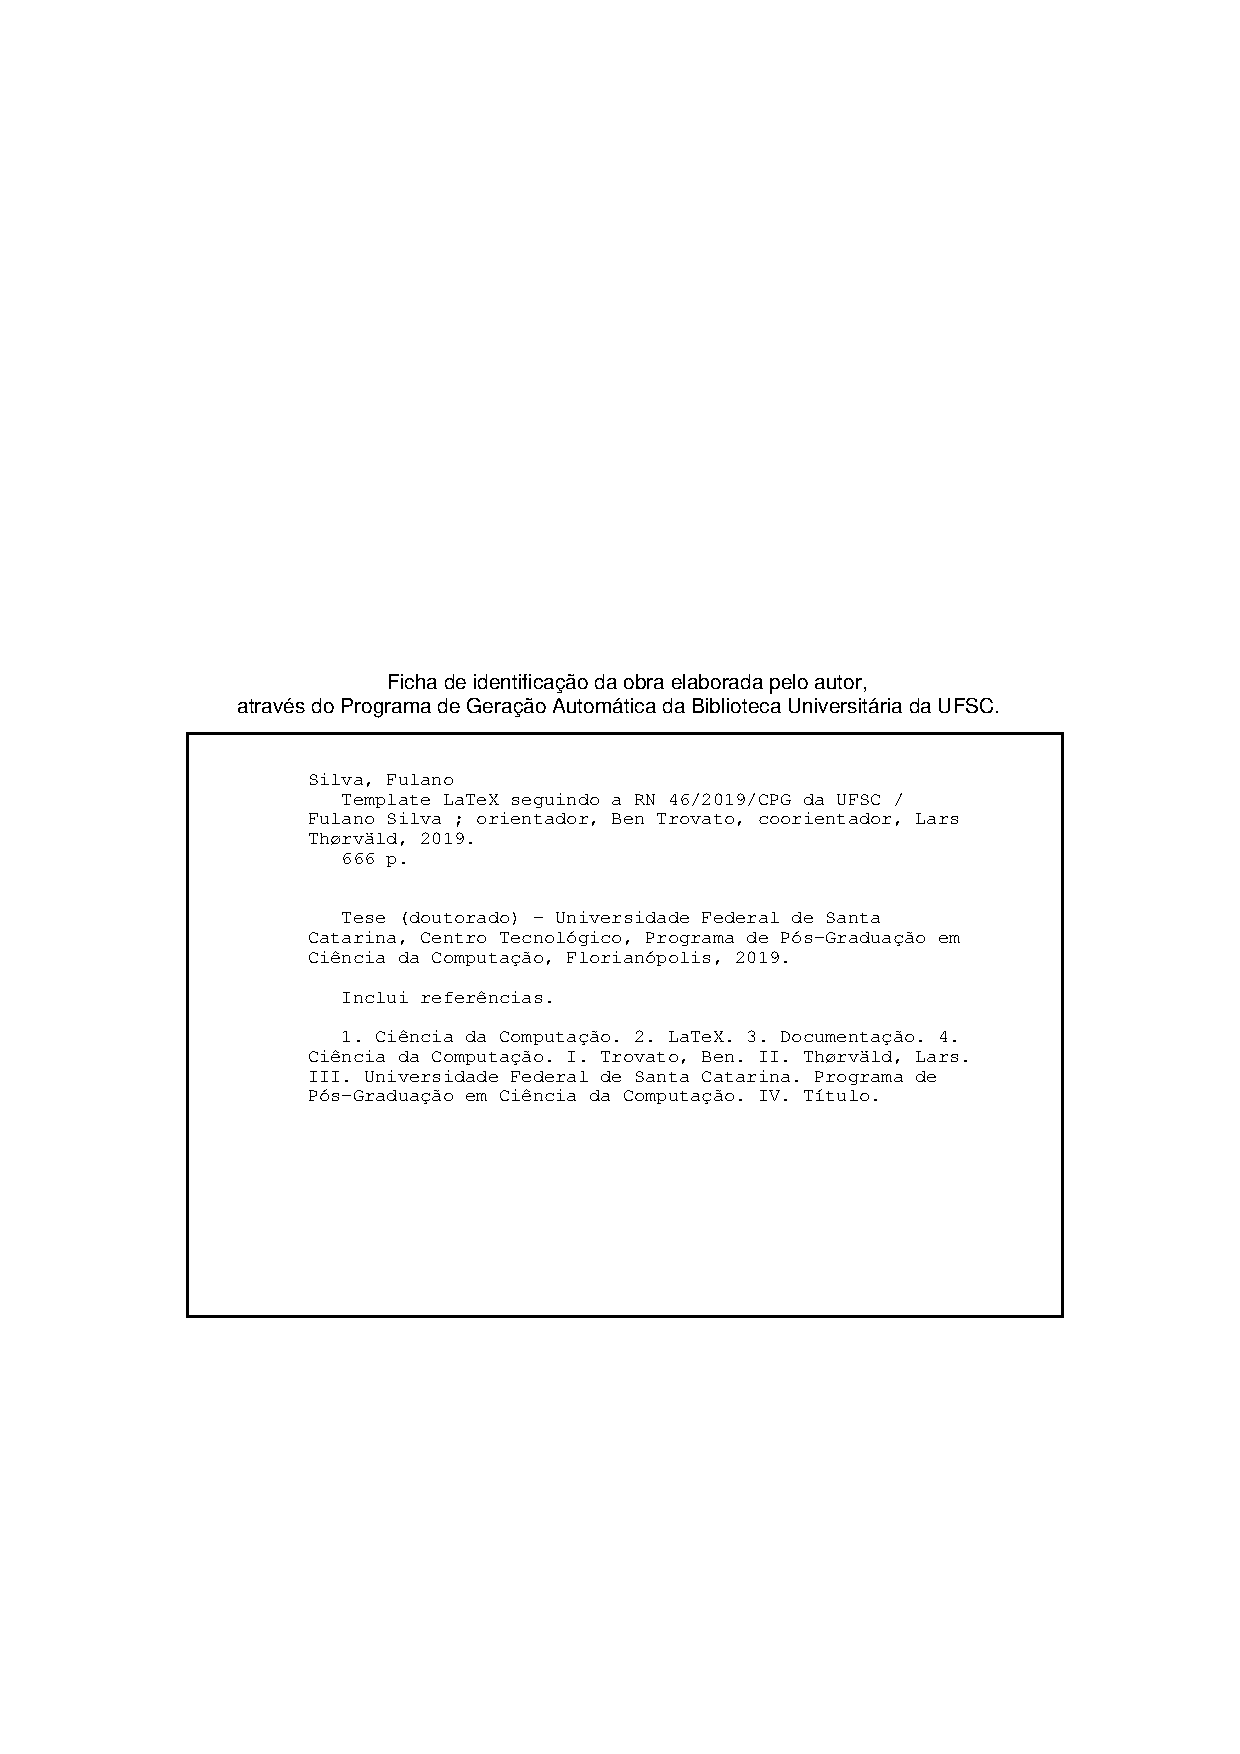
\includepdf{ficha.pdf}
\clearpage
\imprimirfolhadecertificacao
\tableofcontents*%

%%%%%%%%%%%%%%%%%%%%%%%%%%%%%%%%%%%%%%%%%%%%%%%%%%%%%%%%%%%%%%%%%%%%
%%% Corpo do texto                                               %%%
%%%%%%%%%%%%%%%%%%%%%%%%%%%%%%%%%%%%%%%%%%%%%%%%%%%%%%%%%%%%%%%%%%%%
\textual%
\cleardoublepage

\chapter{Introdução}

Bem-vindo ao guia de usuário da classe \mt|ufsc-thesis-rn46-2019|. Essa classe é um conjunto de customizações aplicadas à classe \href{https://ctan.org/pkg/abntex2}{\abnTeX} e ao pacote \mt|abntex2cite|. O objetivo da classe \mt|ufsc-thesis-rn46-2019| é simplório: Adequar o \abnTeX às \href{http://portal.bu.ufsc.br/normalizacao/}{normas emitidas pela Biblioteca Universitária da UFSC} em sequência à \href{https://repositorio.ufsc.br/handle/123456789/197121}{Resolução Normativa nº 46/2019/CPG}.


\section{Autores, suporte e atualizações}

Essa classe foi escrita incialmente por dois alunos do \href{http://ppgcc.posgrad.ufsc.br/}{PPGCC da UFSC}: Alexis Huf e Gustavo Zambonin. Há o risco de esse arquivo não ser atualizado a cada \textit{pull request}, então confira a lista de mártires no GitHub. Essa classe é mantida no no repositório \href{https://github.com/alexishuf/ufsc-thesis-rn46-2019/}{alexishuf/ufsc-thesis-rn46-2019}. Atualizaçãoes podem ser encontradas nesse repositório. \textit{Issues} e PR's são bem vindos.

\subsection{Changelog}

Lista de versões (pelo menos das versões que receberam um número):
\begin{description}
\item[v 0.1-alpha] (\today) Primeiro release para ajudar alunos com pouco prazo de entrega
\end{description}


\section{Quickstart}

A classe \mt|ufsc-thesis-rn46-2019| deveria ser encarada como um drop-in para o \abnTeX. Você pode começar a escrever uma tese do zero usando apenas esta classe, mas talvez você queira usar algum template indicado por algum colega. Na maioria dos casos, bastará usar \mt|\documentclass{ufsc-thesis-rn46-2019/ufsc-thesis-rn46-2019}| supondo que você tenha incluido essa classe via \textit{git submodule} ou tenha copiado o diretório inteiro. 

Esse quickstart assume o caminho não tão rápido, com intuíto de ser didático. Primeiro você precisa da classe. Você pode baixar e extrair o zip, fazer um git clone ou git submodule. Avalie o mais adequado para o seu projeto. Se o seu trabalho for escrito em língua inglesa, você deverá passar uma opção \mt|english| para a classe. Caso contrário não precisa passar nenhuma opção. Logo após chamar a classe, você deverá fornecer dados para a classe (e para o \abnTeX). Veja um preâmbulo completo de exemplo na \autoref{fig:preambulo}. Os próximos parágrafos. Segue um rápido overview sobre o singnificado de cada um dos comandos usados (a maior parte deles continua funcionando como no \abnTeX).

\begin{itemize}
\item \mt|\titulo|, \mt|\autor|, \mt|\instituicao|, \mt|\orientador| e  \mt|\coorientador|: Esses comandos continuam com o mesmo significado e uso que possuiam no \abnTeX;
\item \mt|\data|: As regras da UFSC, exigem que apenas o ano esteja presente na capa e folha de rosto. No entanto, a nova folha de certificação, que é gerada por essa classe precisa da data completa. Forneça a data completa \textbf{em português} (mesmo para documentos em inglês). A classe irá extrair o ano.
\item \mt|\programa| e \mt|\centro|: Nome do Programa de Pós graduação, por extenso e nome do centro (e.g., Centro Tecnológico -- CTC)
\item \mt|\tese| (ou \dissertacao): O texto a ser colocado abaixo do título na folha de rosto tem regras bem definidas. Você deve usar um desses dois comandos para indicar o tipo de trabalho (e consequentemente o nível).
\item \mt|\titulode|: Específica qual é o nome do título almejado. De acordo com a BU, o formato deve sempre ser ``Doutor em XXX'' ou ``Mestre em XXX''.
\item \mt|\preambulo|: Esse comando, fornecido pelo \abnTeX é desnecessário nessa classe. Você pode usar ele para sobreescrever o texto gerado automaticamente a partir do uso de \mt|\tese| e \mt|\titulode|
\end{itemize}

A ``folha de certificação'', que substituiu a antiga folha de arovação agora é gerada em \LaTeX. O nome do orientador já foi fornecido anteriormente, resta apenas indicar os membros avaliadores da banca e o coordenador do programa:
\begin{itemize}
\item \mt|\membrobanca{<nome>}{Universidade}|: Adiciona um membro da banca. \textbf{Atenção}: para membros avaliadores, o ``Dr.'' deve ser inserido após o nome e o ``Prof(a).'' deve preceder o nome.
\item \mt|\coordenador| e \mt|\coordenadora|: Configura o nome do(a) coordenador(a) do Programa de Pós Graduação.
\end{itemize}

\begin{figure}[tb]
  \centering
  \caption{Preambulo de uma tese (ou dissertação) típica usando \mt|ufsc-thesis-rn46-2019|.}
  \label{fig:preambulo}
  \begin{minted}{latex}
\documentclass[english]{ufsc-thesis-rn46-2019/ufsc-thesis-rn46-2019}

% \usepackage's a gosto

\titulo{Template \LaTeX~ seguindo a RN 46/2019/CPG da UFSC}
\autor{Fulano da Silva}
\data{1 de Agosto de 2019}
\instituicao{Universidade Federal de Santa Catarina}
\programa{Programa de Pós-Graduação em Ciências da Computação}
\local{Florianópolis} % Apenas cidade! Sem estado
\tese % ou \dissertacao
\titulode{Doutor em Ciência da Computação}
\orientador{Prof. Dr. Ben Trovato}
\coorientador{Prof. Dr. Lars Thørväld}
\centro{Centro Tecnológico -- CTC}

\membrobanca{Prof. Valerie Béranger, Dr.}{Universidade Federal de Santa Catarina}
\membrobanca{Prof. Aparna Patel, Dr.}{Universidade Federal de Santa Catarina}
\membrobanca{Prof. Huifen Chan, Dr.}{Universidade Federal de Santa Catarina}
\coordenador{Prof. Dr. Charles Palmer, Dr.}
  \end{minted}
  \captionsource{o autor.}
\end{figure}

Os elementos pré-textuais permanecem em grande parte tendo seu comportamento determinado pelo \abnTeX. Alguns elementos, incuídos nesse guia foram alterados para satisfazer normas da UFSC. Esses elementos pré-textuais, também presentes nesse guia são obtidos com o código mostrado na \autoref{fig:pre}. Capa (\imprimircapa) e folha de rosto (\imprimirfolhaderosto*) são obtidas através dos mesmos comandos do \abnTeX, mas agora respeitam as regras da UFSC. 

A ficha catalográfica deve ser gerada em sistema próprio da BU, que produz um PDF. Esse PDF deve ser salvo no seu projeto e incluído no documento utilizando o comando \mt|\includepdf| disponibilizado através de \href{https://www.ctan.org/pkg/pdfpages}{\mt|\usepackage{pdfpages}|}.


\begin{figure}[tb]
  \centering
  \caption{Elementos pré-textuais.}
  \label{fig:pre}
  \begin{minted}{latex}
\pretextual%
\imprimircapa%
\imprimirfolhaderosto*
\clearpage 
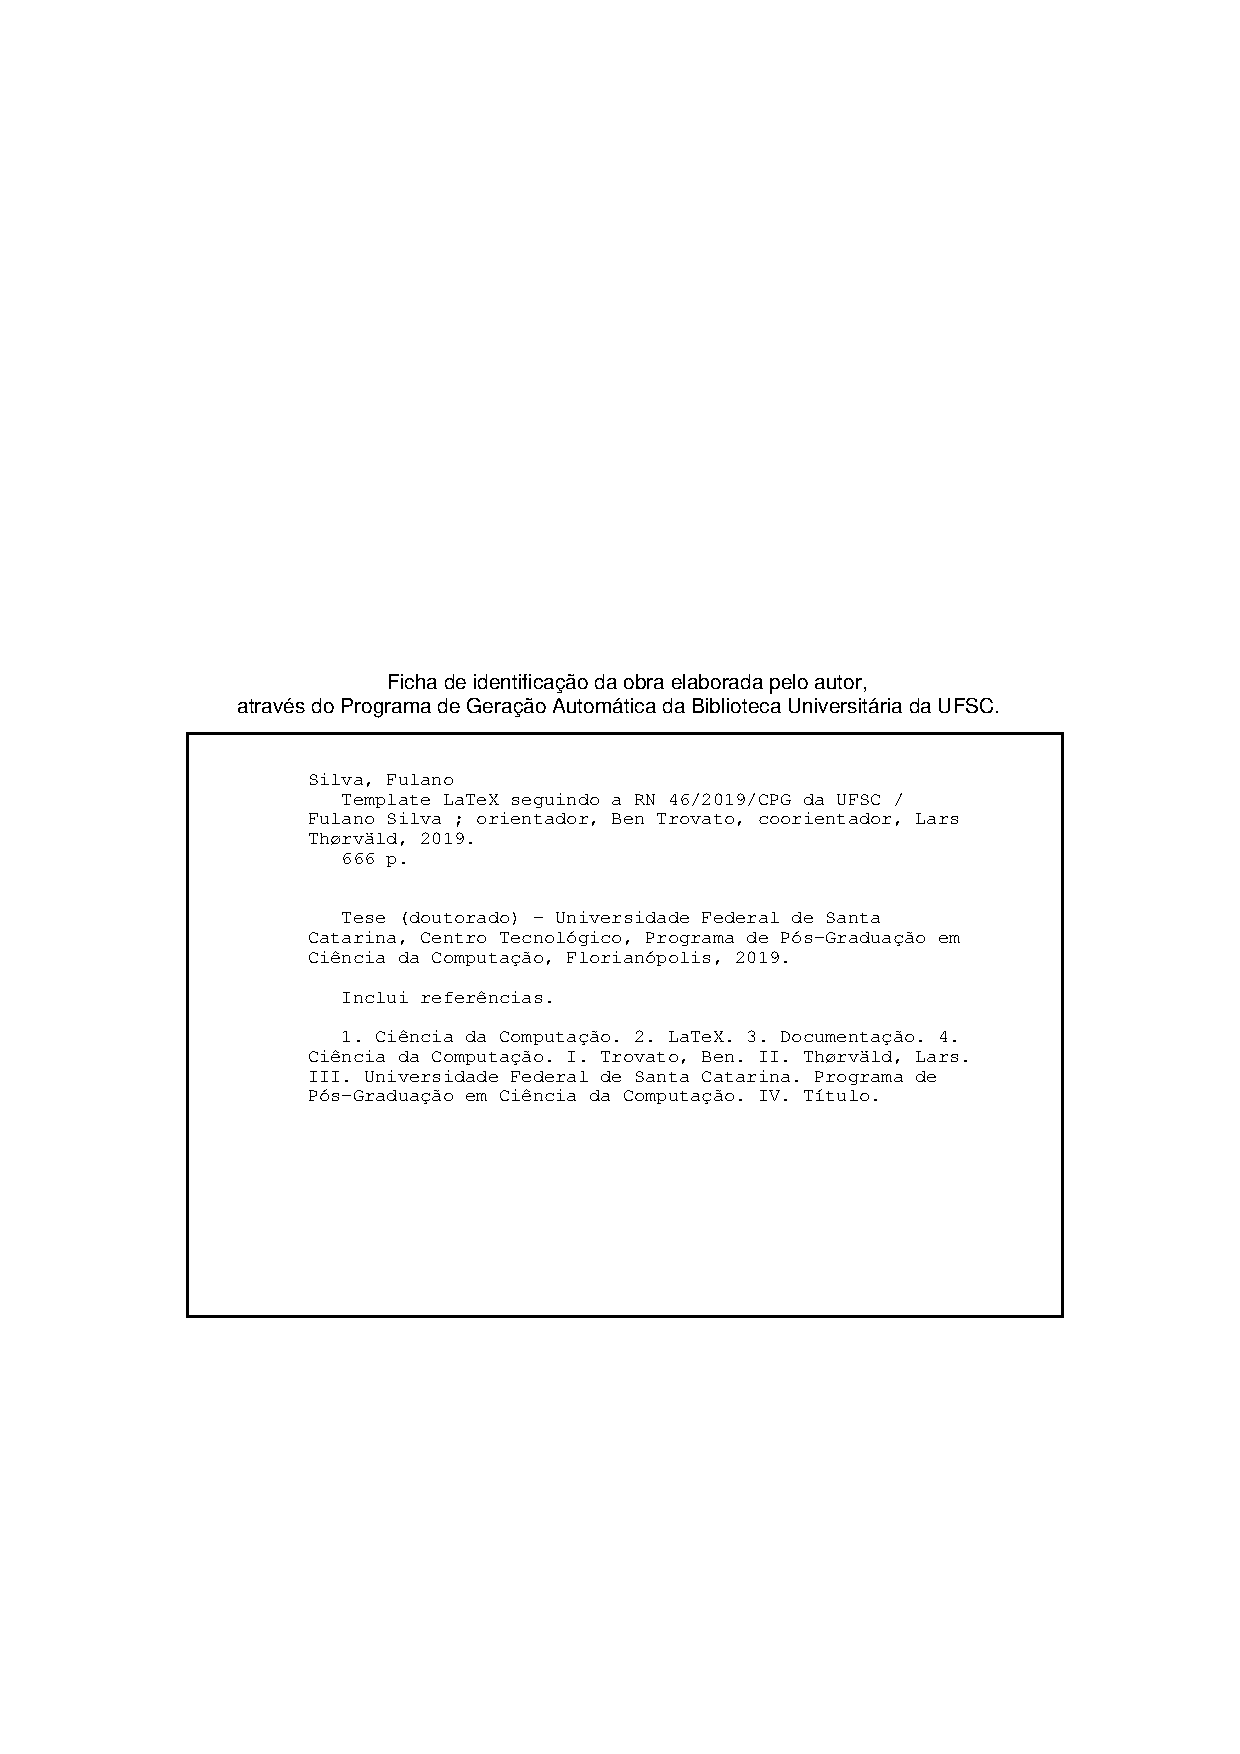
\includepdf{ficha.pdf}
\clearpage
\imprimirfolhadecertificacao
\tableofcontents*%
  \end{minted}
  \captionsource{o autor.}
\end{figure}

Meaningless and wordy sentence with a reference to a seminal article in the hope of averting attention to the lack of content while at the same time borrowing some credibility \cite{turing1937computable}. This harmless sentence tests a nominal reference to \citeonline{dijkstra1968go}.

\begin{itemize}
\item \autoref{ch:bg}
\item \autoref{sec:stuff}
\item \autoref{sec:more}
\item \autoref{sec:yet-more}
\end{itemize}

\lipsum[1]

\chapter{Background}
\label{ch:bg}

\lipsum[1]

\section{Some stuff}
\label{sec:stuff}

\lipsum[1]

\section{Some other stuff}

Atenção! O template da BU deixa figuras e tabelas alinhadas à esquerda. No entanto, o tutorial de Word disponibilizado pela BU diz que Legendas e captions devem respeitar o ``alinhamento da ilustração'' (e apresenta uma ilustração alinhada a esquerda). O tutorial explicando a ABNT mostra uma figura centralizada com legendas alinhadas a esquerda e com recuo até o começo da figura. O autor do .cls se exime de qualquer culpa. Alinhe aqui (com \textbackslash{}centering \textbackslash{}flushright ou \textbackslash{}flushleft) como mandar o seu coração.

\begin{figure}[tb]
  \centering
  \caption{\footnotesize A caption text.}
  \label{fig:f}
  %\lipsum[1]

  <Fig here>
  \captionsource{The author.}
\end{figure}


\subsection{Some more stuff}
\label{sec:more}

\lipsum[1] \footnote{Some footnote}
\footnote{Some Large footnote: \lipsum[4]}

\subsubsection{Yet more stuff}
\label{sec:yet-more}

\lipsum[1]

\subsubsubsection{Yet another more stuff}
\label{sec:yet-another}

\lipsum[1]

%%%%%%%%%%%%%%%%%%%%%%%%%%%%%%%%%%%%%%%%%%%%%%%%%%%%%%%%%%%%%%%%%%%%
%%% Elementos pós-textuais                                       %%%
%%%%%%%%%%%%%%%%%%%%%%%%%%%%%%%%%%%%%%%%%%%%%%%%%%%%%%%%%%%%%%%%%%%%

\postextual
\bibliography{example}

\end{document}
